\documentclass[11pt,a4paper,french,twoside]{PMCours}
\usepackage{hyperref}
%cSpell:ignore thick,fill,yellow,heapsort 
\newcounter{activite}
\newcommand{\activite}{\subsubsection*{Activité~\refstepcounter{activite}\theactivite}}

\begin{document}
\TitreISN{Classe de Terminale}{Année 2021--2022}
{Numérique et Sciences Informatiques}{TP 5 -- Arbres binaires complets - Tas - Tri par tas}


\section{Arbres complet}

\subsection{Définition}

\begin{Definition}{}
    On dit qu'un arbre binaire est \emph{complet} si tous les niveaux 
    sont remplis à l'exception éventuelle du dernier, dans lequel 
    les feuilles sont alignées à gauche.
\end{Definition}


\begin{center}
    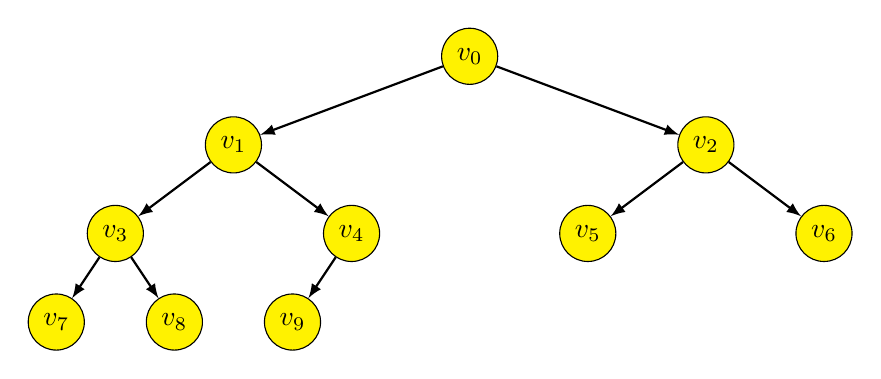
\begin{tikzpicture}[xscale=.5,yscale=.5]
    % Styles (MODIFIABLES)
    \tikzstyle{fleche}=[->,>=latex,thick]
    \tikzstyle{noeud}=[fill=yellow,circle,draw]
    \tikzstyle{feuille}=[fill=orange,circle,draw]
    % Dimensions (MODIFIABLES)
    \def\DistanceInterNiveaux{3}
    \def\DistanceInterFeuilles{2}
    % Dimensions calculées (NON MODIFIABLES)
    \def\NiveauA{(-0)*\DistanceInterNiveaux}
    \def\NiveauB{(-.75)*\DistanceInterNiveaux}
    \def\NiveauC{(-1.5)*\DistanceInterNiveaux}
    \def\NiveauD{(-2.25)*\DistanceInterNiveaux}
    \def\InterFeuilles{(.75)*\DistanceInterFeuilles}
    % Noeuds (MODIFIABLES : Styles et Coefficients d'InterFeuilles)
    \node[noeud] (R0) at ({(0)*\InterFeuilles},{\NiveauA}) {$v_0$};
    \node[noeud] (R1) at ({(-4)*\InterFeuilles},{\NiveauB}) {$v_1$};
    \node[noeud] (R2) at ({(4)*\InterFeuilles},{\NiveauB}) {$v_2$};
    \node[noeud] (R3) at ({(-6)*\InterFeuilles},{\NiveauC}) {$v_3$};
    \node[noeud] (R4) at ({(-2)*\InterFeuilles},{\NiveauC}) {$v_4$};
    \node[noeud] (R5) at ({(2)*\InterFeuilles},{\NiveauC}) {$v_5$};
    \node[noeud] (R6) at ({(6)*\InterFeuilles},{\NiveauC}) {$v_6$};
    \node[noeud] (R7) at ({(-7)*\InterFeuilles},{\NiveauD}) {$v_7$};
    \node[noeud] (R8) at ({(-5)*\InterFeuilles},{\NiveauD}) {$v_8$};
    \node[noeud] (R9) at ({(-3)*\InterFeuilles},{\NiveauD}) {$v_9$};
    % Arcs (MODIFIABLES : Styles)
    \draw[fleche] (R0)--(R1);
    \draw[fleche] (R0)--(R2);
    \draw[fleche] (R1)--(R3);
    \draw[fleche] (R1)--(R4);
    \draw[fleche] (R2)--(R5);
    \draw[fleche] (R2)--(R6);
    \draw[fleche] (R3)--(R7);
    \draw[fleche] (R3)--(R8);
    \draw[fleche] (R4)--(R9);
    \end{tikzpicture}

    \title{Exemple d'arbre binaire complet}
    \end{center}

\begin{Remarque}{}
    Dans un tel arbre, si on numérote les éléments comme dans l'arbre ci-dessus,
    on remarque que $v_3$ a deux fils $v_7$ et $v_8$ et, plus généralement, $v_k$
    a deux fils $v_{2k+1}$ et $v_{2k+2}$.
\end{Remarque}

\begin{Remarque}{}
    Dans un tel arbre, si $h$ est la hauteur et $t$ la taille, on a
    \[2^{h-1}\leq t\leq 2^h-1\]
    Donc
    \[h=\lfloor\log_2(t)\rfloor+1\]
\end{Remarque}

\subsection{Implémentation}

La remarque précédente sur la numérotation des nœuds d'un arbre binaire complet,
nous amène à la possibilité de représenter ce type d'arbre à l'aide d'un tableau.

Ce tableau contient les valeurs de chaque nœud écrits niveau par niveau, 
de gauche à droite. Du coup :
\begin{itemize}
    \item La racine est à l'index $0$.
    \item Le fils gauche du nœud $k$ est le nœud d'index $2k+1$.
    \item Le fils droit du nœud $k$ est le nœud d'index $2k+2$.
    \item Le père du nœud $k$ est le nœud d'index $\left\lfloor\frac{k-1}{2}\right\rfloor$.
\end{itemize}

\begin{Exercice}{}
Créer une class Python nommée \code{ArbreComplet} :
\begin{enumerate}
    \item Le constructeur \code{\_\_init\_\_} ne prend pas d'argument et ne fait que
    créer un attribut \code{L} contenant la liste vide (qui est la représentation
    l'arbre binaire complet).
    \item Ajouter une méthode \code{ajouter(self,valeur)} qui ajoute une feuille
    à l'arbre binaire équilibré (nécessairement à la fin de la liste \code{L}).
    \item Ajouter une méthode \code{est\_vide(self)} qui retourne un booléen.       
    \item Ajouter une méthode \code{fils\_droit(self,k)} qui retourne l'index
    du fils droit du nœud d'index $k$. Ajouter de même, \code{fils\_gauche(self,k)}
    et \code{pere(self,k)}.
    \item Ajouter une méthode \code{valeur(self,k)} qui retourne la valeur du 
    nœud d'index $k$.
\end{enumerate}
On oubliera pas de tester chaque méthode, pour s'assurer de son bon fonctionnement.
\end{Exercice}


\section{Structure de Tas}

\subsection{Définition}

\begin{Definition}{}
    On appelle \emph{tas} un arbre binaire complet dans lequel chaque nœud 
    a une valeur supérieure ou égale à celles de ses deux fils.
\end{Definition}


\begin{center}
    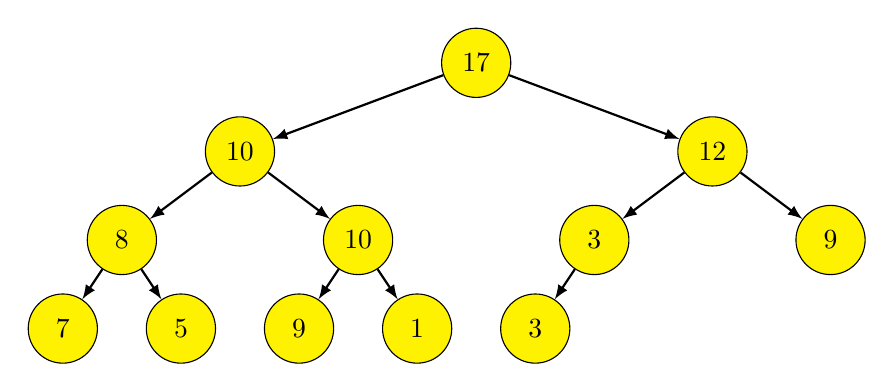
\begin{tikzpicture}[xscale=.5,yscale=.5]
    % Styles (MODIFIABLES)
    \tikzstyle{fleche}=[->,>=latex,thick]
    \tikzstyle{noeud}=[fill=yellow,circle,minimum size=25pt,draw]
    \tikzstyle{feuille}=[fill=orange,circle,minimum size=25pt,draw]
    % Dimensions (MODIFIABLES)
    \def\DistanceInterNiveaux{3}
    \def\DistanceInterFeuilles{2}
    % Dimensions calculées (NON MODIFIABLES)
    \def\NiveauA{(-0)*\DistanceInterNiveaux}
    \def\NiveauB{(-.75)*\DistanceInterNiveaux}
    \def\NiveauC{(-1.5)*\DistanceInterNiveaux}
    \def\NiveauD{(-2.25)*\DistanceInterNiveaux}
    \def\InterFeuilles{(.75)*\DistanceInterFeuilles}
    % Noeuds (MODIFIABLES : Styles et Coefficients d'InterFeuilles)
    \node[noeud] (R0) at ({(0)*\InterFeuilles},{\NiveauA}) {$17$};
    \node[noeud] (R1) at ({(-4)*\InterFeuilles},{\NiveauB}) {$10$};
    \node[noeud] (R2) at ({(4)*\InterFeuilles},{\NiveauB}) {$12$};
    \node[noeud] (R3) at ({(-6)*\InterFeuilles},{\NiveauC}) {$8$};
    \node[noeud] (R4) at ({(-2)*\InterFeuilles},{\NiveauC}) {$10$};
    \node[noeud] (R5) at ({(2)*\InterFeuilles},{\NiveauC}) {$3$};
    \node[noeud] (R6) at ({(6)*\InterFeuilles},{\NiveauC}) {$9$};
    \node[noeud] (R7) at ({(-7)*\InterFeuilles},{\NiveauD}) {$7$};
    \node[noeud] (R8) at ({(-5)*\InterFeuilles},{\NiveauD}) {$5$};
    \node[noeud] (R9) at ({(-3)*\InterFeuilles},{\NiveauD}) {$9$};
    \node[noeud] (R10) at ({(-1)*\InterFeuilles},{\NiveauD}) {$1$};
    \node[noeud] (R11) at ({(1)*\InterFeuilles},{\NiveauD}) {$3$};
    % Arcs (MODIFIABLES : Styles)
    \draw[fleche] (R0)--(R1);
    \draw[fleche] (R0)--(R2);
    \draw[fleche] (R1)--(R3);
    \draw[fleche] (R1)--(R4);
    \draw[fleche] (R2)--(R5);
    \draw[fleche] (R2)--(R6);
    \draw[fleche] (R3)--(R7);
    \draw[fleche] (R3)--(R8);
    \draw[fleche] (R4)--(R9);
    \draw[fleche] (R4)--(R10);
    \draw[fleche] (R5)--(R11);
    \end{tikzpicture}

    \title{Exemple de tas}
    \end{center}

\begin{Remarque}{}
    Dans un tel arbre, la racine contient la valeur maximale.
\end{Remarque}

\begin{Remarque}{}
    Cette structure est très utilisée en informatique, en particulier 
    dans la gestion de fils d'attentes à priorité. Les systèmes d'exploitations
    les utilisent pour les communications hautes performances 
    (qui doivent gérer des messages plus ou moins prioritaires).

    Une autre utilisation est celle du tri par tas, que l'on va voir plus loin.
\end{Remarque}


\subsection{Implémentation}

Il y a deux opérations importantes pour un tas :
\begin{itemize}
    \item \uline{Ajouter une valeur :}
    
    on ajoute la valeur dans l'arbre binaire complet
    (au dernier niveau, en dernière position) puis on le remonte tant qu'il est
    strictement plus grand que son père.
    \item \uline{Retirer la valeur racine :}
    
    on retire le dernier élément du tas
    (au dernier niveau, en dernière position) et on écrase la racine avec.
    Puis, tant qu'il est supérieur à l'un de ses fils, on l'échange avec le plus
    grand de ses deux fils.
\end{itemize}
Ces deux opérations conserve la structure de tas (le semi ordre). De plus, 
elles sont très rapides car elles travaillent sur la hauteur de l'arbre, et non 
pas sur la taille. Leur complexité est donc en $\log_2(t)$. C'est ce qui donne 
tout l'intérêt d'utiliser un tas.

\begin{Exercice}{}
Créer une class Python nommée \code{Tas} :
\begin{enumerate}
    \item Recopier l'intégralité du contenu de la classe \code{ArbreComplet}.
    \item Modifier la méthode \code{ajouter(self,valeur)} pour qu'elle conserve
    la structure de tas (comme précisé ci-dessus).
    \item Ajouter une méthode \code{retirer\_max(self)} qui retourne la valeur racine
    et réorganise le tas comme indiqué ci-dessus.       
\end{enumerate}
On oubliera pas de tester chaque méthode, pour s'assurer de son bon fonctionnement.
\end{Exercice}

\begin{Exercice}{}
    Écrire une fonction \code{maximum(liste)} calcule le maximum de la liste en
    utilisant un tas : elle ajoute un à un tous les éléments de la liste à un tas,
    puis en prends l'élément racine.
\end{Exercice}
    
\section{Tri par tas (heapsort)}

\begin{Methode}{Tri par tas}
Le tri par tas (heapsort) est un algorithme de tri qui se passe en deux phases :
\begin{enumerate}
    \item On créer un tas vide et on lui ajoute, un à un, tous les éléments 
    de la liste à trier.
    \item On retire un à un, tous les éléments du tas pour les remettre dans la
    liste.
\end{enumerate}
Comme on retire à chaque fois le plus grand élément, la liste est triée dans 
l'ordre décroissant. 
\end{Methode}

\begin{Remarque}{}
    Cet algorithme de tri est optimal en nombre de comparaisons et en utilisation 
    mémoire (complexité en $t\log_2(t)$). On peut en faire un tri sur place.

    Malheureusement, il n'optimise pas les caches processeurs et n'est pas 
    parallélisable. Ce qui fait qu'on lui préfère généralement 
    le tri rapide (quicksort).
\end{Remarque}

\begin{Exercice}{}
    Écrire une fonction \code{heapsort(liste)} qui trie la liste dans l'ordre 
    décroissant grâce à l'algorithme du tri par tas.
\end{Exercice}

\begin{Exercice}[(Optimisation)]
    Écrire une fonction \code{heapsort2(liste)} qui fait de même mais en utilisant
    la liste elle même pour y faire grandir et rétrécir le tas. La liste
    sera alors triée dans l'ordre 
    croissant.

    La liste sera, au cours du processus, séparée en deux zones : 
    le début de la liste contient le tas, et la fin qui contient d'abord les 
    éléments pas encore inséré dans le tas, et ensuite les éléments déjà retirés
    du tas.
\end{Exercice}


\end{document}
